\section{Аналитический обзор литературы}
\label{sec:domain}

В данном разделе будет произведён обзор аналитической литературы, необходимой для рассмотрения непосредственно самой темы, нахождение аналогов и нахождение в них проблемных мест; рассмотрены две архитектуры MVC и Redux; рассмотрен серверный движок Node.js и целесообразность его использования в качестве сервера; приведена оценка нерелятивистких баз данных, их преимущества и недостатки.

Также будут рассмотрены основные фреймворки и инструменты, которые будут использованы в рамках дипломного проекта, и произведено сравнение с существующим ПО для решения схожих задач.

\subsection{Дизайн и пользовательский интерфейс}
\label{sub:domain:bayes_net}
Неотъемлимой частью веб-сайта является его представление и дизайн. За все время развития сети Интернет основы дизайна постоянно менялись, однако это помогло выявить некоторые фундаментальные признаки разработки интерфейсов.

Интерфейс пользователя -- это не только его внешний вид. Важной составляющей интерфейса является так называемый <<опыт пользователя>> -- совокупность критериев и факторов, влияющих на взаимодействие пользователя с веб-сайтом. Этими факторами являются краткость и исчерпываемость информации о том, для чего нужен данный сайт; вовлеченность пользователя; однознпрачность и последовательность действий.

Для упрощения разработки таких интерфейсов могут использоваться готовые решения (фреймворки клиентской стороны). Такой подход дает значительное приемущество в скорости разработки, увеличивает переиспользование кода, улучшает его читаемость, а также позволяет получить улучшение производительности засчет внутренних оптимизаций. Также это позволяет сделать веб-сайт единообразным, а следовательно и легко воспринимаемым. Ценой этого является увеличение размера проекта за счет использования сторонних библиотек \cite{framework}.

Ключевым моментом веб-сайта является его наполнение. Веб-страница не должна быть перегружена информацией и в то же время пользователь должен без труда найти все то, что ему нужно. Для поиска лучших вариантов наполнения используется подход A/B-тестирования, когда разным группам пользователей отображается разное содержимое страниц. Данные о поведении этих пользователей сохраняются для дальнейшего анализа и принятия решений о содержимом веб-сайта.

При реализации интерфейса и работе с дизайном мы получаем набор черновиков и дизайнов всех веб-страниц разрабатываемого приложения. Следующим этапом является их преобразование в формат, воспринимаемый современными веб-браузерами. Так как пользователей старых веб-браузеров с каждым годом становится все меньше, акцентировать внимание на их поддержке не стоит. Большинство современных браузеров имеют свои собственные алгоритмы отрисовки содержимого, это следует учитывать при разработке каскадных таблиц стилей. Чтобы избежать проблему портирования стилей, следует использовать фреймворки, ориентированные на особенности каждого веб-браузера.

%О важности вывода структуры (1 стр)

\subsection{Архитектура приложения}
\label{sub:domain:manual_structure}
Архитектура программного обеспечения -- это высокоуровневая структура программной системы, дисциплина создания таких структур и документация по этим структурам. Архитектура является множеством структур, необходимых для рассуждения о программной системе, и включает элементы системы, связи между ними и свойства этих элементов и связей.

Наиболее популярным подходом при проектировании веб-приложений является архитектура MVC \cite{mvc}. Основными преимуществами данного подхода являются:

\begin{itemize}
  \item естественность взаимодействия пользователя с системой: пользователь взаимодействует с представлением, а в ответ получает новое представление с обновленными данными модели;
  \item процесс объединения технологий (таких как базы данных, шаблоны страниц и исполняемый код) упрощается за счет разделения их на разные слои (уровень модели, уровень представления и уровень контроллера);
  \item модели, приближенные к реальным, содержат данные, используемые в бизнес-логике, и операции над ними;
  \item представления, используемые для отображения информации пользователю, которые отделены от слоя бизнес-логики;
  \item контроллеры, используемые для обработки запросов пользователя и формирования ответов пользователю используя представления.
\end{itemize}

С учетом всех приведенных выше дополнительных наблюдений, можно построить вид самой архитектуры, которая приведена на рисунке~\ref{fig:domain:manual_structure:credit_net}.

\begin{figure}[ht]
\centering
  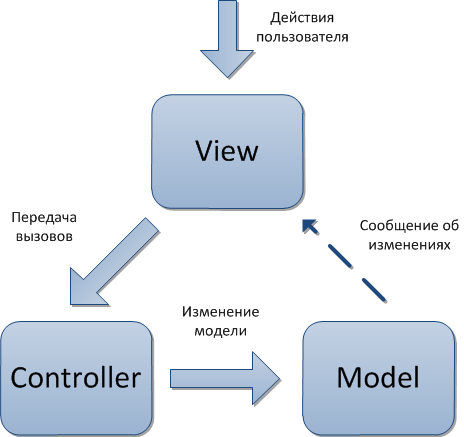
\includegraphics[scale=1]{mvc.png}  
  \caption{ 
  Схема архитектуры MVC }
  \label{fig:domain:manual_structure:credit_net}
\end{figure}

Таким образом, разбиение на уровни является основным преимуществом использования архитектуры MVC. Её применение будет реализовано на серверной стороне.

Со стечением времени, архитектура MVC стала слишком громоздкой и её использование во многих веб-приложениях ориентированных, как клиентское приложение становится уже не целесообразно. На её основе начали создаваться улучшенные виды архитектуры и одна из них является Redux \cite{redux}.

Redux может быть описан тремя фундаментальными принципами:
 
\begin{itemize}
  \item единственный источник правды. Состояние всего приложения сохраняется в дереве объектов одного хранилища. Это дает возможность создавать универсальные приложения. Состояние на сервере может быть сериализовано и отправлено на клиент без особых трудностей;
  \item состояние только для чтения. Единственный способ изменить состояние -- это применить действие, которое описывает, что должно случится;
  \item мутации написаны как простые функции. Для определения того, как дерево состояния будет трансформировано действиями, необходимо писать чистые Reducer-функции. Reducer -- функции, которые берут предыдущее состояние и действие и возвращает обновленное состояние. Чистая функция -- это функция, которая является детерминированной и не обладает побочными эффектами.
\end{itemize}

\begin{figure}[ht]
\centering
  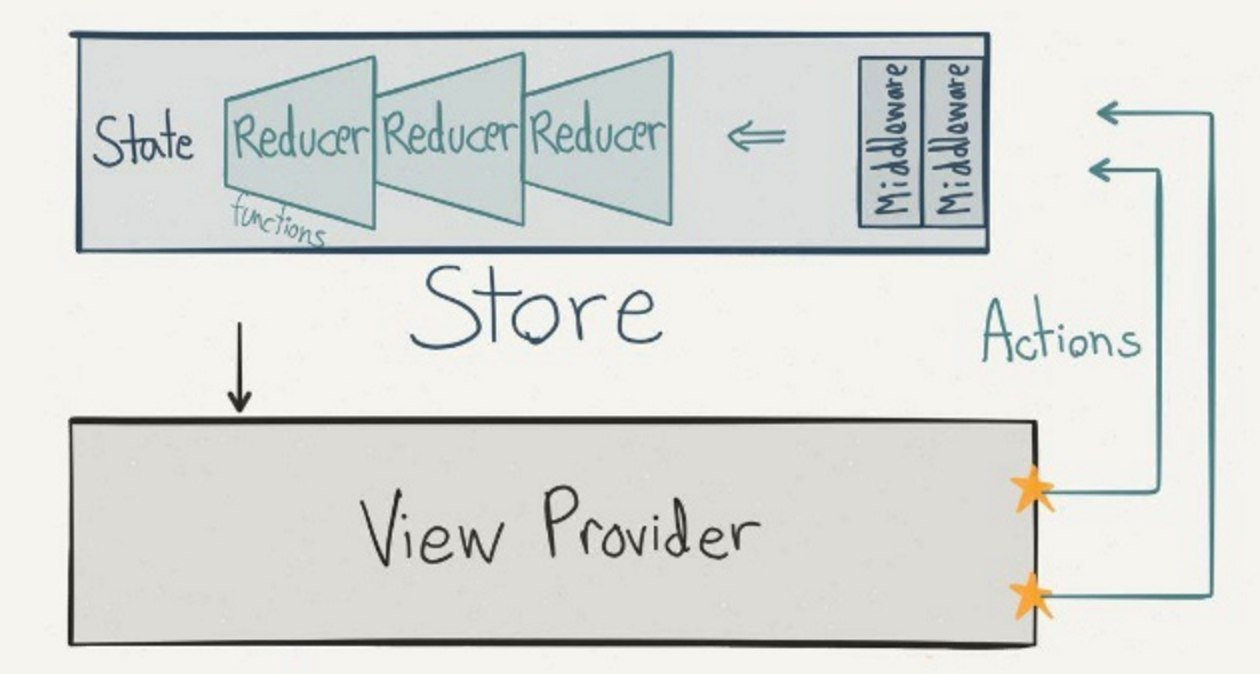
\includegraphics[scale=0.3]{redux.jpg}  
  \caption{ Схема архитектуры Redux }
  \label{fig:domain:manual_structure:credit_redux}
\end{figure}

На рисунке~\ref{fig:domain:manual_structure:credit_redux}. показана основная схема архитектуры. Разберемся с основными её частями.

Действия -- это структура, которая передает данные из вашего приложения в хранилище. Они являются единственными источниками информации для хранилища.

Редьюсер -- это чистая функция, которая принимает предыдущее состояние и действие (state и action) и возвращает следующее состояние (новую версию предыдущего) \cite{redux_framework}.

Хранилище -- это объект, который соединяет эти части вместе. Хранилище берет на себя следующие задачи:
\begin{itemize}
  \item содержит состояние приложения (application state);
  \item предоставляет доступ к состоянию с помощью getState();
  \item предоставляет возможность обновления состояния с помощью встроенной функции dispatch(action);
  \item регистрирует слушатели (listeners) c помощью subscribe(listener).
\end{itemize}

Таким образом, единственный Store и использование чистых функций является основным преимуществом использования архитектуры Redux.

%Указание что это NP трудная задача (0.5)
%Табличка с оценкой количества сетей в зависимости от числа переменных (для устрашения) (0.2)

\subsection{Серверная платформа и база данных}
\label{sub:domain:mdl_principle}
Node.js является серверной технологией, которая основана на разработанном компанией Google JavaScript-движке V8. Это масштабируемая система, поддерживающая не программные потоки или отдельные процессы, а асинхронный ввод-вывод, управляемый событиями. Она идеально подходит для веб-приложений, которые не выполняют сложных вычислений, но к которым происходят частые обращения \cite{node_js}.

При использовании обычного веб-сервера, например Apache, при каждом запросе веб-ресурса для обслуживания этого запроса сервер создает отдельный программный поток или вызывает новый процесс. Даже если сервер реагирует на запросы достаточно быстро, а после удовлетворения запроса все приводит в порядок, при таком подходе задействуется множество ресурсов. В результате у наиболее популярных веб-приложений возникают предпосылки для серьезных проблем производительности \cite{apache}.

В отличие от этого Node не создает новый программный поток или процесс для каждого запроса, а прослушивает конкретные события, и когда эти события происходят, соответствующим образом на них реагирует. Node не блокирует никаких запросов, дожидаясь завершения действий, инициируемых событием, а сами события обрабатываются в относительно простом цикле обработки событий по принципу <<первым пришел -- первым обслужен>>.

Node-приложения создаются с помощью языка JavaScript (или альтернативных языков, компилирующихся в JavaScript), который ничем не отличается от языка, применяемого в приложениях на стороне клиента. Однако в отличие от языка JavaScript, используемого в браузере, для Node нужно создать среду разработки. Node можно установить на платформе Unix/Linux, Mac OS или Windows \cite{js}.

Рассмотрим работу обычного веб-сервера, например Apache. Apache поддерживает две модели мультипроцессорной обработки поступающих запросов. В первой для каждого запроса выделяется отдельный процесс, продолжающийся до тех пор, пока запрос не будет обслужен, во второй для каждого запроса выделяется отдельный программный поток.

В первой MPM-модели, известной как модель prefork, может создаваться столько дочерних процессов, сколько указано в конфигурационном файле Apache. Преимущество создания отдельного процесса состоит в том, что приложения, к которым обращаются посредством запроса, например PHP-приложения, не обязательно должны быть многопоточными. Недостаток заключается в том, что каждый процесс расходует память, и эта модель характеризуется неважной масштабируемостью.

Во второй MPM-модели, известной как модель worker, реализуется гибридная схема процесс-поток, когда каждый поступающий запрос обрабатывается с помощью нового программного потока. С точки зрения расхода памяти этот подход более эффективен, но он требует, чтобы все приложения были многопоточными (то есть были безопасными в отношении потоков). Хотя популярный язык создания веб-приложений PHP теперь безопасен в отношении потоков, нет никаких гарантий, что множество различных библиотек, используемых с интерпретатором этого языка, также безопасно в отношении потоков.

Независимо от используемой модели, запросы обрабатываются в параллельном режиме. Если к веб-приложению в одно и то же время обращается пять человек и сервер имеет соответствующую настройку, все пять запросов обрабатываются одновременно.

В Node все происходит по-другому. При запуске Node-приложения создается единственный программный поток. Node-приложение выполняется в этом потоке в ожидании, что некое приложение сделает запрос. Когда Node-приложение получает запрос, никакие другие запросы не обрабатываются до тех пор, пока не завершится обработка текущего запроса.

Все это кажется не слишком эффективным, если бы не то обстоятельство, что Node работает в асинхронном режиме, используя цикл обработки событий и функции обратного вызова. Цикл обработки событий просто опрашивает конкретные события и в нужное время вызывает обработчики событий. В Node таким обработчиком событий является функция обратного вызова.

В отличие от других однопоточных приложений, к Node-приложению делается запрос, оно должно, в свою очередь, запросить какие-то ресурсы (например, обратиться к базе данных или получить доступ к файлу). В этом случае Node инициирует запрос, но не ожидает ответа на этот запрос. Вместо этого запросу назначается некая функция обратного вызова. Когда запрошенное будет готово (или завершено), генерируется событие, активизирующее соответствующую функцию обратного вызова, призванную что-то сделать либо с результатом запрошенного действия, либо с запрошенными ресурсами.

Если пять человек обращаются к Node-приложению в одно и то же время и приложению нужно обратиться к ресурсам из файла, для каждого запроса Node назначает свою функцию обратного вызова событию ответа. Когда для каждого из них ресурс становится доступен, вызывается нужная функция обратного вызова, и запрос удовлетворяется. В промежутке Node-приложение может обрабатывать другие запросы либо для того же приложения, либо для какого-нибудь  другого.

NoSQL -- ряд подходов, направленных на реализацию хранилищ баз данных, имеющих существенные отличия от моделей, используемых в традиционных реляционных СУБД с доступом к данным средствами языка SQL. Применяется к базам данных, в которых делается попытка решить проблемы масштабируемости и доступности за счёт атомарности и согласованности данных \cite{nosql}.

В реляционной модели база состоит из таблиц, которые состоят из строк и колонок. У каждой колонки есть свой тип данных (строка, число, логическое значение, дата, текст, бинарный блоб). Все строки однотипны.

Обычно каждый вид объектов хранится в отдельной таблице. Обычно у каждого объекта есть уникальный идентификатор. Идентификатор может быть как условным, то есть просто числом, так и вытекающим из предметной области.

Серверы реляционных БД обеспечивают стандартные операторы доступа к данным в таблицах, такие как SELECT, INSERT, UPDATE и DELETE. Разные серверы предоставляют также некоторые дополнительные операторы. Извлекать данные из таблиц можно по множеству различных критериев.

NoSQL -- это отход от реляционной модели в пользу более специфических моделей данных. Например, традиционно успешными NoSQL-системами являются системы хранения пар <<ключ-значение>>, документные хранилища и графовые базы данных.

У NoSQL обычно перечисляют следующие достоинства:
\begin{itemize}
  \item масштабируемость. Горизонтальное масштабирование существующих традиционных СУБД обычно является трудоемкой, дорогостоящей и эффективной только до определенного уровня задачей. В то же время многие NoSQL-решения проектировались исходя из необходимости масштабироваться горизонтально и делать это <<на лету>>. Поэтому эта процедура обычно проще и прозрачнее в NoSQL, чем в РСУБД;
  \item производительность БД на одном узле, а не в кластере также является немаловажным параметром. Для многих задач такие свойства традиционных СУБД, как транзакционность, изолированность изменений, надежность в пределах одного узла или даже сама реляционная модель, не всегда нужны в полном объеме. Поэтому отказ от этих свойств (всех или некоторых) позволяет NoSQL иногда добиваться большей производительности на одном узле, чем традиционным решениям;
  \item надежная работа в условиях, когда отказ железа или сетевая недоступность -- обычное дело, является одним из свойств многих решений NoSQL. Основной способ ее обеспечения -- это репликация. Сама по себе репликация отнюдь не является уникальной особенностью NoSQL, но здесь, как и при масштабировании, важную роль играют эффективность и легкость внесения изменений в существующую инсталляцию. Переход БД к работе в режиме репликации -- это простая задача для большинства NoSQL-решений;
  \item простота разработки и администрирования -- также важный аргумент в пользу NoSQL-технологий. Целый ряд задач, связанных с масштабированием и репликацией, представляющих значительную сложность и требующих обширной специальной экспертизы на традиционных СУБД, у NoSQL занимает считанные минуты. Задачи установки и настройки, само использование NoSQL-решений обычно существенно проще и менее трудоемки, чем в случае с РСУБД. Поэтому NoSQL-системы стали очевидным выбором для многих проектов, где скорость разработки и внедрения является ключевым фактором.
\end{itemize}

%Оценка апостериорных вероятностей (K2) (2-3)

\subsection{Клиентские фреймворки и платформы}
\label{sub:domain:other_algos}
React.js -- фреймворк для создания интерфейсов от Facebook. React построен на парадигме реактивного программирования. Этот декларативный подход предлагает описывать данные в виде набора утверждений или формул. Изменение одного из параметров ведёт за собой автоматический пересчёт всех зависимостей. Работа с DOM в браузере часто оказывается источником проблем с производительностью. Создатели React решили проблему радикально. Ребята написали реализацию DOM на JavaScript. Фреймворк использует её, чтобы при изменении состояния компонент судить о том, что поменять в реальном DOM и как сделать это эффективно \cite{react_js}.

Apache Cordova -- это платформа разработки мобильных приложений с открытым исходным кодом. Она позволяет использовать стандартные веб-технологии, такие как HTML5, CSS3 и JavaScript для кроссплатформенной разработки, избегая родного языка разработки для каждой из мобильных платформ. Приложения выполняются внутри обертки нацеленной на каждую платформу и полагаются на стандартные API для доступа к датчикам устройства, данным и состоянию сети \cite{cordova}.

Приложения Cordova полагаются на общий файл config.xml, который содержит информацию о приложении и определяет параметры, влияющие на то как приложенеи работает, такие как, реагирует ли оно на изменение ориентации устройства. Этот файл соответствует спецификации W3C Упакованные веб-приложения, или widget.

Само приложение реализована как веб-страницы, по умолчанию локальный файл под названием index.html, который ссылается на любой CSS, JavaScript, изображения, файлы мультимедиа или другие ресурсы необходимы для его запуска. Приложение выполняет как WebView в пределах оболочки приложения, которую вы распространяете в магазины приложений.

WebView с поддержкой Cordova может представлять приложения и полностью его пользовательский интерфейс. На некоторых платформах она также может быть компонентом в больших, гибридные приложения, который объединяют WebView с другими компонентами приложения.

Интерфейс плагина доступен для Cordova и других компоненты, для взаимодействия друг с другом. Это позволяет вызывать код на языке платформы из JavaScript. В идеале на нескольких платформах устройств согласуются JavaScript API, чтобы этот машинный код. Начиная с версии 3.0 плагины предоставляют привязки к стандартным API интерфейсам устройства. Сторонние плагины предоставляют дополнительные привязки для функции не обязательно доступных на всех платформах.

Начиная с версии 3.0 можно использовать два основных рабочих процесса для создания мобильных приложений: кроссплатформенный рабочий процесс и платформо-ориентированный процесс разработки. 

Кросс платформенный рабочий процесс формируется возле утилиты cordova, также известном как Cordova CLI, который был введен начиная с Cordova 3.0. CLI это высоко уровневый инструмент который позволяет построить проекты для как можно большего количества платформа одновременно, абстрагируя как можно больше функциональности низкоуровневых скриптов. 

Платформо-ориентированный рабочий процесс опирается на набор скриптов более низкого уровня, которые приспособлены для каждой поддерживаемой платформы и отдельную утилита Plugman, которая позволяет применять плагины индивидуально к выбранной платформе.

\subsection{Обзор существующих программ} % (fold)
\label{sub:domain:existing_programs}
Существует много приложений, в основе работы которых лежит инструменты личного мониторинга здоровья. В основе этих инструментов может лежать как и веб-ориентированное приложения, так и десктопные приложения. Рассмотрим наиболее популярные из них.

Приняв во внимание тему дипломного проекта, наибольший интерес в существуем ПО будет представлять функциональность возможность работы с большим количеством данных.
Ниже рассматриваются некоторые из программ.

\subsubsection{МедАрхив}

Проект организован с целью информационной поддержки медицинского обслуживания. Медархив -- это web-площадка для обмена медицинской информацией между врачами и медицинскими учреждениями, с одной стороны, и пациентами, с другой. Работа Медархива ориентирована на потребности тех, кто лечит, и тех, кто лечится.

Пациент и врач могут взаимодействовать через Медархив почти так же, как реальном мире. Пациент рассказывает о проблеме, врач дает рекомендации, отправляет на обследование, ставит диагноз. Личная медицинская информация, включая консультации врача, электронную медицинскую карту, надежно и конфиденциально хранится в архиве пациента.

Достоинства:
\begin{itemize}
  \item удобная панель навигации. Она позволяет быстро найти необходимый пункт;
  \item быстрый просмотр сведений. Возможность просматривать информацию о себе, о врачах;
  \item организация расписания. Позволяет не только смотреть за расписанием определенных врачей. Но и организовывать собственное расписание;
  \item онлайн консультация, а также онлайн запись на прием к врачу.
\end{itemize}

Недостатки:
\begin{itemize}
  \item отсутсивие кроссплатформенности;
  \item недоступность утилит для автоматизации создания встреч;
  \item нет возможности следить за своим ребенком. Нужно создавать отдельный аккаунт.
\end{itemize}
\begin{figure}[ht]
\centering
  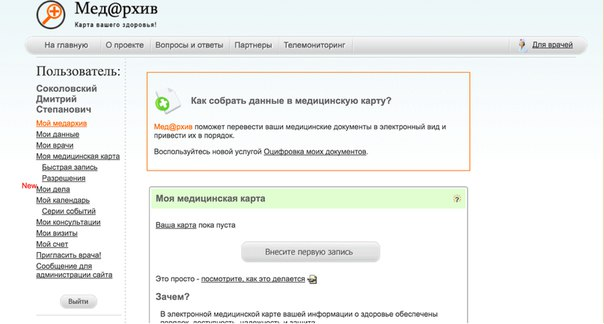
\includegraphics[scale=0.7]{medAr.jpg}  
  \caption{ Главная страница пациента приложения МедАрхив }
  \label{fig:domain:manual_structure:credit_med}
\end{figure}

\subsubsection{HealthKit}

Приложение под продукцию Apple. На первый взгляд в нём сложно разобраться. HealthKit -- это платформа, которая будет собирать информацию о вашем состоянии не только на основе датчиков одного трекера, а отовсюду, откуда это только возможно. Из приложений, которые установлены на вашем iPhone и iPad, из фитнес-устройств. Таким образом HealthKit будет выдавать полную картинку о вашем состоянии. Мало того, в iOS 8 приложения смогут обмениваться информацией с HealthKit, чтобы сделать тренировки эффективнее или подкоректировать диету.

Достоинства:
\begin{itemize}
  \item большие возможности кастомизации;
  \item есть возможность анализировать график анализа жизненных покозателей;
  \item удобный интерфейс пользователя.
\end{itemize}

Недостатки:
\begin{itemize}
  \item избыточная сложность;
  \item не кроссплатформенность;
  \item нет возможность расшарить данные врачу или медцентру.
\end{itemize}

\begin{figure}[ht]
\centering
  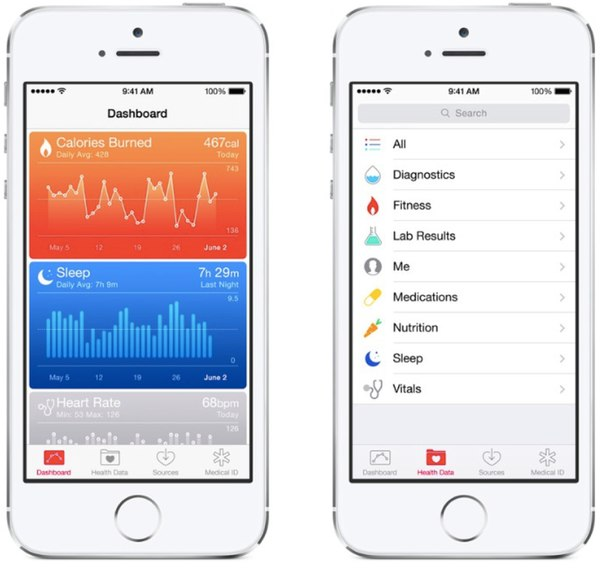
\includegraphics[scale=0.7]{healthkit.jpg}  
  \caption{ Приложение HealthKit }
  \label{fig:domain:manual_structure:credit_healthkit}
\end{figure}

\subsubsection{OnDoc}

OnDoc -- новый бесплатный веб-сервис и мобильное приложение (iOS, Android) для хранения персональных медицинских данных. Вы можете добавлять записи о результатах посещения врача и проведенных обследованиях. Тут же можно записаться на прием в любую из 4 тыс. клиник-партнеров сервиса. После приема в партнерских клиниках информация об обследовании, диагнозе и лечении появляются в профиле автоматически. Можно предоставить онлайн доступ другому врачу к своим данным. Также приложение может напоминать о приеме лекарств и дозировке, выдавать персональные рекомендации по снижению риска возможных заболеваний. Разработчики утверждают, что вся информация в сервисе хранится в зашифрованном виде в соответствии с 152 ФЗ <<О персональных данных>>. 

Достоинства:
\begin{itemize}
  \item легкий интерфейс;
  \item кроссплатформенность;
  \item возможность выбора нескольких клиник или медцентров;
  \item возможность организовывать прием медицинских препаратов;
  \item возможность анализировать состояние здоровья за определенный срок.
\end{itemize}

Недостатки:
\begin{itemize}
  \item отсутсвует календарь;
  \item нет полноценного функционала импорта/экспорта;
  \item нет доступа к полноценной кастомизации.
\end{itemize}


\subsection{Обоснование выбора языка и среды разработки} % (fold)
\label{sub:domain:existing_language}

\subsubsection{Язык разработки}

Исходные коды программного средства должны быть реализованы на языке программирования JavaScript. Обусловлен этот выбор следующими критериями:

\begin{itemize}
  \item язык JavaScript -- язык программирования с динамической типизацией, позволяющей писать более краткий и лаконичный код;
  \item встроенная поддержка юникода в строках;
  \item JavaScript не вынуждает писать код в определенном стиле и парадигме
  \item автоматическая сборка мусора;
  \item кроссплатформенность, подразумевающая, что программное средство, написанное на языке программирования JavaScript, будет функционировать одинаково, вне зависимости от операционной системы и браузера;
  \item JavaScript является мультипарадигменным языком, что позволяет использовать различные решения, лучше подходящие для данной задачи;
  \item большое количество библиотек;
  \item возможность использовать JavaScript как на сервере, так и на клиенте;
  \item широкая распространенность JavaScript, что позволит разобраться в коде большему количеству разработчиков без предварительной подготовки.
\end{itemize}

В качестве интегрированной среды разработки программного средства должно быть использовано программное обеспечение JetBrains WebStorm \cite{webstorm}. Он имеет ряд преимуществ:
\begin{itemize}
  \item возможность работы под различными операционными системами;
  \item встроенный отладчик для языка платформы Node.js;
  \item поддержка систем контроля версий;
  \item статический анализ кода, подсветка синтаксиса и ошибок;
  \item навигация по проекту и исходному коду.
\end{itemize}

\subsubsection{Выбор платформы серверной разработки}

Серверная сторона приложения разработана с использованием платформы Node.JS.
Node.js -- программная платформа, основанная на движке V8 (транслирующем JavaScript в машинный код), превращающая JavaScript из узкоспециализированного языка в язык общего назначения. Node.js добавляет возможность JavaScript взаимодействовать с устройствами ввода-вывода через свой API (написанный на C++), подключать другие внешние библиотеки, написанные на разных языках, обеспечивая вызовы к ним из JavaScript-кода. Node.js применяется преимущественно на сервере, выполняя роль веб-сервера, но есть возможность разрабатывать на Node.js и десктопные оконные приложения (при помощи NW.js, AppJS или Electron для Linux, Windows и Mac OS) и даже программировать микроконтроллеры (например, tessel и espruino). В основе Node.js лежит событийно-ориентированное и асинхронное (или реактивное) программирование с неблокирующим вводом/выводом.

\subsubsection{Выбор СУБД}

MongoDb -- это документо-ориентированная база данных. Означает, что каждая запись это документ, без жестко заданной схемы, который может содержать вложенные документы \cite{mongodb}.

MongoDb хороша высокой скоростью записи/чтения, масштабированностью, но опять же сохранность и целостность данных не так хороша. Так, например, в Монго есть отличная реализация репликации, которая довольно легко устанавливается и настраивается или же шардинг (возможность разнести данные по нескольким серверам), который тоже довольно прост в установке. В комплексе, можно получить систему распределенных вычислений с высокой отказоустойчивостью.

MongoDb использует JSON нотацию для хранения и управления документами, а также свой достаточно удобный язык запросов.

Основные возможности данной СУБД:
\begin{itemize}
  \item документо-ориентированное хранилище (простая и мощная JSON-подобная схема данных);
  \item достаточно гибкий язык для формирования запросов;
  \item динамические запросы;
  \item полная поддержка индексов;
  \item профилирование запросов;
  \item быстрые обновления <<на месте>>;
  \item эффективное хранение двоичных данных больших объёмов;
  \item журналирование операций, модифицирующих данные в БД;
  \item поддержка отказоустойчивости и масштабируемости.
\end{itemize}

\subsubsection{ORM Mongoose}

В данном проекте будет использоваться Mongoose. Mongoose -- это библиотека Node.js, которая предоставляет возможность отображения, схожего со знакомым интерфейсом внутри Node.js. Mongoose переводит данные в базу данных объектов JavaScript для дальнейшего их использования вашим приложением.

\subsection{Постановка задачи}
\label{sub:domain:task}
В результате выполнения дипломного проекта должно быть разработано мобильное приложение, написанное на языке JavaScript, для ведение анализа состояния о пациенте, путем сохранения информации о обследованиях со следующими спецификациями:
\begin{itemize}
  \item разрабатываемое ПО должно иметь возможность запускаться под платформами Android 5.0, iOS 7.0;
  \item разрабатываемое ПО должно позволять возможность создавать вручную заключения полученные от медучреждений;
  \item разрабатываемое ПО должно позволять возможность сканирование фотографий заключений медучреждений;
  \item разрабатываемое ПО должно позволять возможность экспортировать в PDF документ информацию с сохраненных заключений медицинского обследования;
  \item время работы ПО должно быть приемлемым.
\end{itemize}